\subsection{Memory Management} \label{memmanagement}
As the OS is targered to build safe-critical embedded applications, dynamic memory allocation its not allowed for the kernel design, because can lead to out-of-storage run-time failures, which are undesirable. However, some applications can be easily deployed using this allocation scheme, so a safe and portable implementation becomes relevant in the scope of the user-code. 

In a typical C environment, memory can be allocated using the standard library functions  \textit{malloc()} and \textit{free()}, but they may not be suitable in most embedded applications because they are not always available on small microcontrollers or their implementation can be relatively large, taking up valuable code space. Also, there is a range of unspecified and implementation-defined behaviour associated with dynamic memory allocation, as well as a number of other potential pitfalls. Additionally, some implementations can suffer from fragmentation.

To get around this problem, the OS provides its own memory-management interface for dynamic allocation as a fully kernel-independent extension. When the application requires RAM, instead of calling \textit{malloc()},  call \lstinline{qMalloc()} \index{\lstinline{qMalloc}}. When RAM is being freed, instead of calling \textit{free()}, use \lstinline{qFree()} \index{\lstinline{qFree}}. Both functions have the same prototype as the standard C library counterparts.

\subsubsection{Principle of operation}
The allocation scheme works by subdividing a static array into smaller blocks and using the \textit{First-Fit} approach (see figure \ref{fig:memman}). 

\begin{figure}[H]
    \centering
    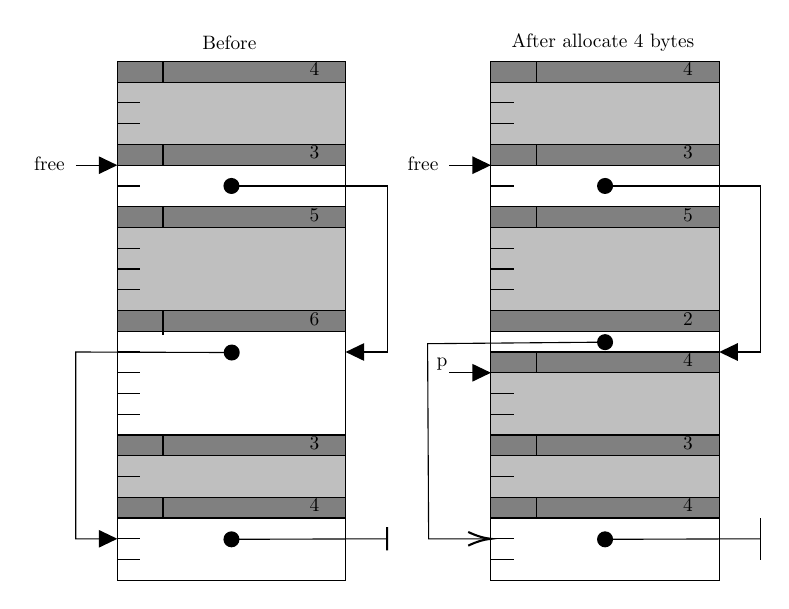
\begin{tikzpicture}[x=0.75pt,y=0.75pt,yscale=-1,xscale=1]
        \foreach \x in {20,60,90,140,200,230}{
            \draw  [fill=gray  ,fill opacity=1 ] (100,\x) -- (210,\x) -- (210,\x+10) -- (100,\x+10) -- cycle ;
        }
        
        \draw  [fill=lightgray  ,fill opacity=1 ] (100,30) -- (210,30) -- (210,60) -- (100,60) -- cycle ;
        \draw  [fill=white ,fill opacity=1 ] (100,70) -- (210,70) -- (210,90) -- (100,90) -- cycle ;
        \draw  [fill=lightgray ,fill opacity=1 ] (100,100) -- (210,100) -- (210,140) -- (100,140) -- cycle ;
        \draw  [fill=white  ,fill opacity=1 ] (100,150) -- (210,150) -- (210,200) -- (100,200) -- cycle ;
        \draw  [fill=lightgray  ,fill opacity=1 ] (100,210) -- (210,210) -- (210,230) -- (100,230) -- cycle ;
        \draw  [fill=white  ,fill opacity=1 ] (100,240) -- (210,240) -- (210,270) -- (100,270) -- cycle ;
        
        \foreach \x in {20,60,90,140,160,200,230}{
            \draw  [fill=gray  ,fill opacity=1 ] (280,\x) -- (390,\x) -- (390,\x+10) -- (280,\x+10) -- cycle ;
        }

        \draw  [fill=lightgray  ,fill opacity=1 ] (280,30) -- (390,30) -- (390,60) -- (280,60) -- cycle ;
        \draw  [fill=white  ,fill opacity=1 ] (280,70) -- (390,70) -- (390,90) -- (280,90) -- cycle ;
        \draw  [fill=lightgray  ,fill opacity=1 ] (280,100) -- (390,100) -- (390,140) -- (280,140) -- cycle ;
        \draw  [fill=white  ,fill opacity=1 ] (280,150) -- (390,150) -- (390,160) -- (280,160) -- cycle ;
        \draw  [fill=lightgray  ,fill opacity=1 ] (280,210) -- (390,210) -- (390,230) -- (280,230) -- cycle ;
        \draw  [fill=white  ,fill opacity=1 ] (280,240) -- (390,240) -- (390,270) -- (280,270) -- cycle ;
        \draw  [fill=lightgray ,fill opacity=1 ] (280,170) -- (390,170) -- (390,200) -- (280,200) -- cycle ;

        \foreach \x in {40,50,...,260}{
            \draw    (100,\x) -- (111,\x) ;
            \draw    (280,\x) -- (291,\x) ;
        }        
        
        \foreach \x in {20,60,90,160,200,230}{ \draw    (302,\x) -- (302,\x+10) ; }
        \foreach \x in {20,60,90,200,230}{ \draw    (122,\x) -- (122,\x+10) ; }
        
        \draw  (260,170) -- (278,170) ;
        \draw  (80,70) -- (98,70) ;
        \draw  (155,250.25) -- (230,250) ;
        \draw  (335,250.25) -- (410,250) ;
        \draw  (410,240) -- (410,260) ;        
        \draw  (260,70) -- (278,70) ;
        \draw  (122,140) -- (122,152) ;
        \draw  (155,80) -- (230,80) -- (230,160) -- (212,160) ;
        \draw  (335,155.25) -- (249.5,156) -- (250,250) -- (278,250) ;
        \draw  (335,80) -- (410,80) -- (410,160) -- (392,160) ;
        \draw  (155.13,160.25) -- (80,160) -- (80,250) -- (98,250) ;
        
        \draw [shift={(210,160)}, rotate = 360] [fill=black  ][line width=0.75]  [draw opacity=0] (8.93,-4.29) -- (0,0) -- (8.93,4.29) -- cycle;
        \draw [shift={(155,80)}, rotate = 0] [color=black  ][fill=black  ][line width=0.75] (0, 0) circle [x radius= 3.35, y radius= 3.35];
        \draw [shift={(100,250)}, rotate = 180] [fill=black  ][line width=0.75]  [draw opacity=0] (8.93,-4.29) -- (0,0) -- (8.93,4.29) -- cycle;
        \draw [shift={(155.13,160.25)}, rotate = 180.19] [color=black][fill=black ][line width=0.75](0, 0) circle [x radius= 3.35, y radius= 3.35];
        \draw [shift={(100,70)}, rotate = 180] [fill=black  ][line width=0.75]  [draw opacity=0] (8.93,-4.29) -- (0,0) -- (8.93,4.29) -- cycle;
        \draw [shift={(230,250)}, rotate = 539.81] [color=black  ][line width=0.75]    (0,5.59) -- (0,-5.59);
        \draw [shift={(155,250.25)}, rotate = 359.81] [color=black][fill=black ][line width=0.75] (0, 0) circle [x radius= 3.35, y radius= 3.35];
        \draw [shift={(390,160)}, rotate = 360] [fill=black ][line width=0.75]  [draw opacity=0] (8.93,-4.29) -- (0,0) -- (8.93,4.29) -- cycle;
        \draw [shift={(335,80)}, rotate = 0] [color=black ][fill=black ][line width=0.75] (0, 0) circle [x radius= 3.35, y radius= 3.35];
        \draw [shift={(280,70)}, rotate = 180] [fill=black ][line width=0.75]  [draw opacity=0] (8.93,-4.29) -- (0,0) -- (8.93,4.29) -- cycle;
        \draw [shift={(335,250.25)}, rotate = 359.81] [color=black][fill=black ][line width=0.75] (0, 0) circle [x radius= 3.35, y radius= 3.35];
        \draw [shift={(280,170)}, rotate = 180] [fill=black ][line width=0.75] [draw opacity=0] (8.93,-4.29) -- (0,0) -- (8.93,4.29) -- cycle;
        \draw [shift={(280,250)}, rotate = 180] [color=black ][line width=0.75] (10.93,-3.29) .. controls (6.95,-1.4) and (3.31,-0.3) .. (0,0) .. controls (3.31,0.3) and (6.95,1.4) .. (10.93,3.29);
        \draw [shift={(335,155.25)}, rotate = 179.5] [color=black ][fill=black ][line width=0.75] (0, 0) circle [x radius= 3.35, y radius= 3.35];
        
        \draw (67.33,69.33) node [scale=0.7] [align=left] {free};
        \draw (247.33,69.33) node [scale=0.7] [align=left] {free};
        \draw (256.5,166) node [scale=0.7] [align=left] {p};
        \draw (154,11) node [scale=0.7] [align=left] {Before};
        \draw (334,11) node [scale=0.7] [align=left] {After allocate 4 bytes};
        
        \foreach \x/\y in {24/4,64/3,94/5,144/6,204/3,234/4}{ \draw (195,\x) node [scale=0.7] [align=left] {\y}; }
        \foreach \x/\y in {24/4,64/3,94/5,144/2,164/4,204/3,234/4}{ \draw (375,\x) node [scale=0.7] [align=left] {\y}; }
    \end{tikzpicture}
    \caption{First-fit allocation policy}
    \label{fig:memman}
\end{figure}

If adjacent free blocks are available, the implementation combines them into a single larger block, minimizing the risk of fragmentation, making it suitable for applications that repeatedly allocate and free different sized blocks of RAM.

\begin{tcolorbox}
\ArrowBoldDownRight \textit{Note}: Because memory is statically declared, it will make the application appear to consume a lot of RAM, even before any memory has been allocated from it.
\end{tcolorbox}

\begin{tcolorbox}
\AsteriskBold \textit{Warning}: All the memory management APIs are NOT interrupt-safe. Use these APIs only from the base context.
\end{tcolorbox}

\begin{tcolorbox}
\AsteriskBold \textit{Warning}: The application is not exempt from memory leaks if the user does not perform adequate memory management. Here, the worst case scenario can occur in the absence of free memory. 
\end{tcolorbox}

\subsubsection{Memory pools}

A memory pool its a special resource that allows memory blocks to be dynamically allocated from a user-designated memory region. Instead of typical pools with fixed-size block allocation, the pools in QuarkTS can be of any size, thereby the user is responsible for selecting the appropriate memory pool to allocate data with the same size. 

The \textit{default} memory management unit resides in a memory pool object. Also called the \textit{default pool}. The total amount of available heap space in the default memory pool is set by \lstinline{Q_DEFAULT_HEAP_SIZE}, which is defined in \lstinline{qconfig.h}.

Besides the \textit{default} pool, any number of additional memory pools can be defined. Like any other object in QuarkTS, memory pools are referenced by handles, a variable of type \lstinline{qMemMang_Pool_t} \index{\lstinline{qMemMang_Pool_t}} and should be initialized before use with the \lstinline{qMemMang_Pool_Setup()} \index{\lstinline{qMemMang_Pool_Setup}} API function.
\medskip

\begin{lstlisting}[style=CStyle]
qBool_t qMemMang_Pool_Setup( qMemMang_Pool_t * const mPool, void* Area, 
                             size_t size )
\end{lstlisting}

\subsubsection*{Parameters}
\begin{itemize}
    \item \lstinline{mPool} : A pointer to the memory pool instance. 
    \item \lstinline{Area} :  A pointer to a memory region (\lstinline{qUINT8_t}) statically allocated to act as Heap of the memory pool. The size of this block should match the \lstinline{size} argument.
    \item \lstinline{size} : The size of the memory block pointed by \lstinline{Area}. 
\end{itemize}

To perform operations in another memory pool, besides the \textit{default} pool, an explicit switch should be performed using \lstinline{qMemMang_Pool_Select()} \index{\lstinline{qMemMang_Pool_Select}}. Here, a pointer to the target pool should be passed as input argument.  From now on, every call to \lstinline{qMalloc()}, or \lstinline{qFree()} will run over the newly selected memory pool. To return to  the \textit{default pool},  a new call to  \lstinline{qMemMang_Pool_Select()} is required passing \lstinline{NULL} as input argument. 
\medskip

\begin{lstlisting}[style=CStyle]
qBool_t qMemMang_Pool_Select( qMemMang_Pool_t * const mPool )
\end{lstlisting}

To keep track of the memory usage, the \lstinline{qMemMang_Get_FreeSize()} \index{\lstinline{qMemMang_Get_FreeSize}} API function returns the number of free bytes in the memory pool at the time the function is called.
\medskip

\begin{lstlisting}[style=CStyle]
size_t qMemMang_Get_FreeSize( void )
\end{lstlisting}

\subsubsection*{Usage example:}

\lstinputlisting[style=CStyle]{sec3memmangdem1.c}